\documentclass[10pt, a4paper, onecolumn]{scrartcl}
\usepackage{cite}  
\usepackage{times}
\usepackage{amsmath}
\usepackage{amsfonts}
\usepackage{amssymb}
\usepackage{graphicx}
\usepackage{listings}
\usepackage{enumitem} % used for list - no spaces between items
\usepackage[english]{babel} % English language/hyphenation
\usepackage[top=2cm, bottom= 3.2cm, left=2cm, right=2cm, columnsep=0.6cm]{geometry}
\usepackage{color} %red, green, blue, yellow, cyan, magenta, black, white
\definecolor{mygreen}{RGB}{28,172,0} % color values Red, Green, Blue
\definecolor{mylilas}{RGB}{170,55,241}
\usepackage{fancyhdr}
\pagestyle{fancyplain}
\fancyhead{}
\renewcommand{\headrulewidth}{0pt} % Remove header underlines
\fancyfoot[L]{} % Empty left footer
\fancyfoot[C]{} % Empty center footer
\fancyfoot[R]{\thepage} 
\usepackage{tikz}
\usetikzlibrary{shapes.geometric,arrows}

\usepackage{sectsty} % Allows customizing section commands
\sectionfont{\centering\large\textbf}
\subsectionfont{\flushleft\normalsize\normalfont\textbf}
\subsubsectionfont{\flushleft\normalsize\normalfont\textit}
%\allsectionsfont{\centering} % Make all sections centered

\setlength\parindent{0pt} % remove all indentations in document

%----------------------------------------------------------------------------------------
%	BEGIN DOCUMENT
%----------------------------------------------------------------------------------------
\newcommand{\horrule}[1]{\rule{\linewidth}{#1}}

\begin{document}
	
	\title{\normalfont \normalsize
		\textsc{University of Witwatersrand, Department of Electrical Engineering} \\ [10pt]
		\horrule{0.5pt} \\ [10pt]
		\huge Shopping Route Recommender \\ Sprint Planning Document \\
		\horrule{2pt} \\ [10pt]}
	\author{\textbf{\normalsize{Luka Cakic (671913), Ronen Freeman (386910), Devin Taylor (603956) and Matthew Marsden (609293)}} \\ [10pt]}
	\date {\normalsize \today}
	
	\maketitle
	
	\section{Software Development Life-Cycle Model}
	
		The life-cycle model that the group collectively decided upon are the agile models. The primary motivation for this decision is that changes in project requirements and deliverables during development of such a project in inevitable. In addition, the project is developed based on customer collaboration and not on a contractual negotiation. An agile method was preferred to that of the Waterfall method due to the possibility of the project having rapidly changing requirements based on customer desirables as well as there being tight time constraints suggesting that incrementation development would be preferable over a sequential development process. In addition, as a result of the project requirement potentially changing throughout development, the sequentiality of the Waterfall model cannot be followed, as a result of this model following a method whereby the project requirements are fully defined and known in advance. For these stated reasons the chosen life-cycle model is that of an agile approach. 
		
		\subsection{SCRUM}
		
			In order for Shopping Route Recommender to be a user interactive application, the development team has approached the application's development and aspects as potential users themselves. In effect, this allows "users" to work continuously within the development team, with continuous considerations made towards end user interests. As a result of this, the development process is a team-based approach. The control of conflicting ideas, needs and interests must therefore be adequately managed due to the close collaboration of each development team member. The co-operation amongst the team must be maximised, and communication is vital for successful completion of project tasks. For the reasons stated, the chosen agile process is the SCRUM method. Taking all the aforementioned considerations into account, the SCRUM method ultimately allows a team to maximise productivity.  The fact that there are multiple developers working on the project it is necessary to divide up the work ensuring a faster completion time. In order to do this multiple aspects of this project will be developed in parallel. As a result of this the constant feedback for development sprints, proposed by the SCRUM method, provide additional motivation for the selection of the SCRUM method.
		
	\section{SCRUM Roles}
	
		\subsection{Product Owner}
		
			As there is no direct interfacing with a client in this project there is no need to dedicate a specific group member to being the product owner. As an alternative to this, the team will function collectively as the product owner and will therefore decide as a group what should be placed in the sprint backlog. In addition, the team will in unison negotiate a release date for the product. The feature and priority adjustments will also be collectively decided. 
			
		\subsection{Scrum Master}
		
			The Scrum master for the project will be Devin Taylor. This is primarily due to this members ability to manage time efficiently and work efficiently with a team. He is the most influential group member capable of presenting and inflicting  managerial decisions. As a direct result he also ensures the team is fully functional and that there exists close co-operation across all team roles and functions. He is also capable of representing the management of the project if necessary.  
			
		\subsection{Development Team}
		
			All group members will form part of the group of developers. The main reason for this is due to the limited number of group members available thus the consideration of delivery date is a priority. Therefore, Luka Cakic, Matthew Marsden, Ronen Freeman and Devin Taylor will all form an integral part of the developer team. As Devin Taylor is also the Scrum master, the time dedicated to developing will be less than that of the remaining group members. All the members are cross-functional and demonstrate the necessary skills to complete the web application. Some of the development roles include the programming, testing and customer needs analysis of the project. 
	
	\section{SCRUM Planning}
	
		One of the ways in which the group plans on both implementing and monitoring the SCRUM method is through an application called Trello. Trello forms an important backbone to the structure of the SCRUM method planning, by providing a carded system whereby jobs are divided amongst cards and the development team selects cards from this stack and completes its defined task. The cards can be taken by individual group members and upon completetion of the tasks on the card, the member updates the progress of the task. In doing so, the other group members are informed of all the individual member's project progress. A screen shot of the board currently being used can be seen below. 
		
		\begin{figure}[h!]
			\centering
			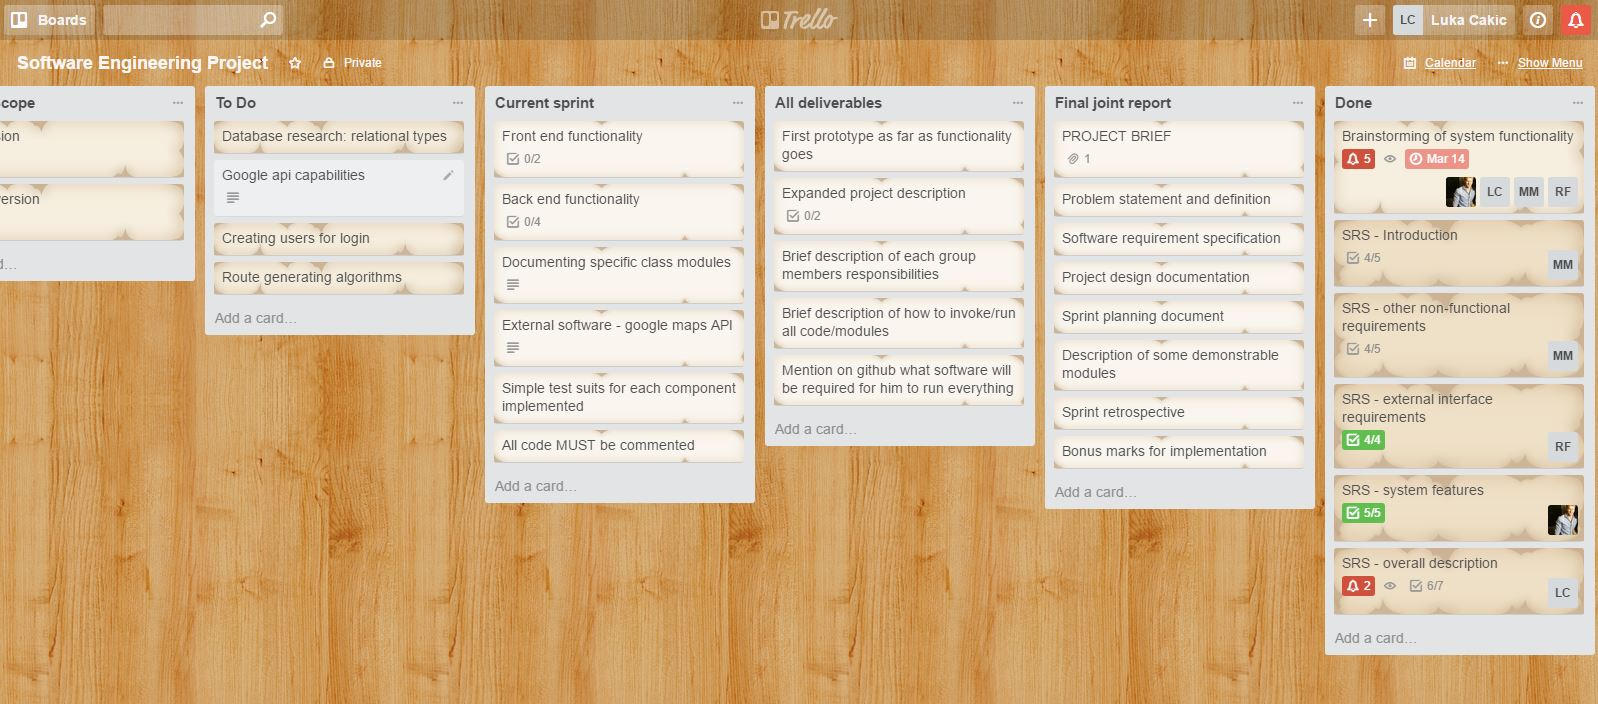
\includegraphics[scale = 0.4]{Images/Trello.jpg}
			\caption{Trello board used for project development}
			\label{menu}
		\end{figure}
		
		
	
	
\end{document}